
\documentclass[border=8pt, multi, tikz]{standalone} 
\usepackage{import}
\subimport{../../../tools/PlotNeuralNet/layers/}{init}
\usetikzlibrary{positioning}
\usetikzlibrary{3d} %for including external image 

\usetikzlibrary{calc,decorations.pathreplacing,fit}
\def\IOColor{rgb:white,4;black,1}
\def\ConvColor{rgb:yellow,5;red,2.5;white,5}
\def\ActColor{rgb:yellow,5;red,5;white,5}
\def\PoolColor{rgb:red,1;black,0.3}
\def\UpColor{rgb:blue,2;green,1;black,0.3}
\def\CopyColor{rgb:white,1;black,3}
\def\OutColor{rgb:magenta,5;black,7}
\def\GraphColor{rgb:blue,5;green,2.5;white,5}
\def\GraphActColor{rgb:blue,5;green,5;white,3}
\def\SumColor{rgb:blue,5;green,15}
\def\DCColor{rgb:red,2;blue,5;white,2}
\def\HLCCColor{rgb:green,3;blue,1;white,8}

\newcommand{\copymidarrow}{\tikz \draw[-Stealth,line width=0.8mm,draw={rgb:blue,4;red,1;green,1;black,3}] (-0.3,0) -- ++(0.3,0);}

\begin{document}
\begin{tikzpicture}
\tikzstyle{connection}=[ultra thick,every node/.style={sloped,allow upside down},draw=\edgecolor,opacity=0.7]
\tikzstyle{copyconnection}=[ultra thick,every node/.style={sloped,allow upside down},draw={rgb:blue,4;red,1;green,1;black,3},opacity=0.7]

\tikzstyle{bus}=[ultra thick,-Stealth,draw={rgb:blue,4;red,1;green,1;black,3},opacity=0.7,rounded corners=4pt]
\tikzstyle{op}=[draw=black!60,fill=\HLCCColor,rounded corners=3pt,align=flush center,font=\small,inner sep=4pt]

\pic[shift={(0,0,0)}] at (0,0,0)
    {Box={name=in,
        caption={},
        xlabel={{"",}},
        zlabel={},
        fill=\IOColor,
        opacity=0.6,
        height=40.0,
        width=0.4,
        depth=27.8}};

\begin{scope}[shift={(in-east)}]
    \node[canvas is zy plane at x=0,transform shape,inner sep=0pt] at (0,0)
        {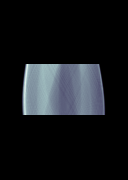
\includegraphics[width=5.560cm,height=8.000cm]{sinograms/incomplete.png}};
\end{scope}

\node[below=12pt,align=center,font=\small] at (in-nearsoutheast) {\textbf{Incomplete $y$}\\$180\times128$};

\pic[shift={(2.2,0,0)}] at (in-east)
    {RightBandedBox={name=enc0,
        caption={},
        xlabel={{"32","32",}},
        zlabel={$184\times128$},
        fill=\ConvColor,
        bandfill=\ActColor,
        opacity=0.4,
        height=40.0,
        width={3.75,3.75},
        depth=27.8}};

\draw [connection]  (in-east)    -- node {\midarrow} (enc0-west);

\pic[shift={(0,0,0)}] at (enc0-east)
    {Box={name=pool0,
        caption={},
        xlabel={{"",}},
        zlabel={},
        fill=\PoolColor,
        opacity=0.5,
        height=30.0,
        width=1,
        depth=20.9}};

\pic[shift={(1.2,0,0)}] at (pool0-east)
    {RightBandedBox={name=enc1,
        caption={},
        xlabel={{"64","64",}},
        zlabel={$92\times64$},
        fill=\ConvColor,
        bandfill=\ActColor,
        opacity=0.4,
        height=30.0,
        width={4.5,4.5},
        depth=20.9}};

\draw [connection]  (pool0-east)    -- node {\midarrow} (enc1-west);

\pic[shift={(0,0,0)}] at (enc1-east)
    {Box={name=pool1,
        caption={},
        xlabel={{"",}},
        zlabel={},
        fill=\PoolColor,
        opacity=0.5,
        height=22.5,
        width=1,
        depth=15.7}};

\pic[shift={(1.2,0,0)}] at (pool1-east)
    {RightBandedBox={name=enc2,
        caption={},
        xlabel={{"128","128",}},
        zlabel={$46\times32$},
        fill=\ConvColor,
        bandfill=\ActColor,
        opacity=0.4,
        height=22.5,
        width={5.25,5.25},
        depth=15.7}};

\draw [connection]  (pool1-east)    -- node {\midarrow} (enc2-west);

\pic[shift={(0,0,0)}] at (enc2-east)
    {Box={name=pool2,
        caption={},
        xlabel={{"",}},
        zlabel={},
        fill=\PoolColor,
        opacity=0.5,
        height=16.9,
        width=1,
        depth=11.8}};

\pic[shift={(1.2,0,0)}] at (pool2-east)
    {RightBandedBox={name=enc3,
        caption={Bottleneck},
        xlabel={{"256","256",}},
        zlabel={$23\times16$},
        fill=\ConvColor,
        bandfill=\ActColor,
        opacity=0.4,
        height=16.9,
        width={6.0,6.0},
        depth=11.8}};

\draw [connection]  (pool2-east)    -- node {\midarrow} (enc3-west);

\pic[shift={(1.2,0,0)}] at (enc3-east)
    {Box={name=up2,
        caption={},
        xlabel={{"128",}},
        zlabel={},
        fill=\UpColor,
        opacity=0.5,
        height=22.5,
        width=5.25,
        depth=15.7}};

\pic[shift={(0,0,0)}] at (up2-east)
    {Box={name=copy2,
        caption={},
        xlabel={{"128",}},
        zlabel={},
        fill=\CopyColor,
        opacity=0.25,
        height=22.5,
        width=5.25,
        depth=15.7}};

\pic[shift={(0,0,0)}] at (copy2-east)
    {RightBandedBox={name=dec2,
        caption={},
        xlabel={{"128","128",}},
        zlabel={},
        fill=\ConvColor,
        bandfill=\ActColor,
        opacity=0.4,
        height=22.5,
        width={5.25,5.25},
        depth=15.7}};

\draw [connection]  (enc3-east)    -- node {\midarrow} (up2-west);

\path (enc2-southeast) -- (enc2-northeast) coordinate[pos=1.25] (enc2-top) ;
\path (copy2-south)  -- (copy2-north)  coordinate[pos=1.25] (copy2-top) ;
\draw [copyconnection]  (enc2-northeast)  
-- node {\copymidarrow}(enc2-top)
-- node {\copymidarrow}(copy2-top)
-- node {\copymidarrow} (copy2-north);

\pic[shift={(1.2,0,0)}] at (dec2-east)
    {Box={name=up1,
        caption={},
        xlabel={{"64",}},
        zlabel={},
        fill=\UpColor,
        opacity=0.5,
        height=30.0,
        width=4.5,
        depth=20.9}};

\pic[shift={(0,0,0)}] at (up1-east)
    {Box={name=copy1,
        caption={},
        xlabel={{"64",}},
        zlabel={},
        fill=\CopyColor,
        opacity=0.25,
        height=30.0,
        width=4.5,
        depth=20.9}};

\pic[shift={(0,0,0)}] at (copy1-east)
    {RightBandedBox={name=dec1,
        caption={},
        xlabel={{"64","64",}},
        zlabel={},
        fill=\ConvColor,
        bandfill=\ActColor,
        opacity=0.4,
        height=30.0,
        width={4.5,4.5},
        depth=20.9}};

\draw [connection]  (dec2-east)    -- node {\midarrow} (up1-west);

\path (enc1-southeast) -- (enc1-northeast) coordinate[pos=1.25] (enc1-top) ;
\path (copy1-south)  -- (copy1-north)  coordinate[pos=1.25] (copy1-top) ;
\draw [copyconnection]  (enc1-northeast)  
-- node {\copymidarrow}(enc1-top)
-- node {\copymidarrow}(copy1-top)
-- node {\copymidarrow} (copy1-north);

\pic[shift={(1.2,0,0)}] at (dec1-east)
    {Box={name=up0,
        caption={},
        xlabel={{"32",}},
        zlabel={},
        fill=\UpColor,
        opacity=0.5,
        height=40.0,
        width=3.75,
        depth=27.8}};

\pic[shift={(0,0,0)}] at (up0-east)
    {Box={name=copy0,
        caption={},
        xlabel={{"32",}},
        zlabel={},
        fill=\CopyColor,
        opacity=0.25,
        height=40.0,
        width=3.75,
        depth=27.8}};

\pic[shift={(0,0,0)}] at (copy0-east)
    {RightBandedBox={name=dec0,
        caption={},
        xlabel={{"32","32",}},
        zlabel={},
        fill=\ConvColor,
        bandfill=\ActColor,
        opacity=0.4,
        height=40.0,
        width={3.75,3.75},
        depth=27.8}};

\draw [connection]  (dec1-east)    -- node {\midarrow} (up0-west);

\path (enc0-southeast) -- (enc0-northeast) coordinate[pos=1.25] (enc0-top) ;
\path (copy0-south)  -- (copy0-north)  coordinate[pos=1.25] (copy0-top) ;
\draw [copyconnection]  (enc0-northeast)  
-- node {\copymidarrow}(enc0-top)
-- node {\copymidarrow}(copy0-top)
-- node {\copymidarrow} (copy0-north);

\pic[shift={(1.2,0,0)}] at (dec0-east)
    {Box={name=head,
        caption={},
        xlabel={{"1",}},
        zlabel={},
        fill=\OutColor,
        opacity=0.6,
        height=40.0,
        width=0.8,
        depth=27.8}};

\pic[shift={(1.6,0,0)}] at (head-east)
    {Ball={name=sum,
        fill=\SumColor,
        opacity=0.6,
        radius=2.5,
        logo={$+$},
        caption={}}};

\pic[shift={(1.6,0,0)}] at (sum-east)
    {Ball={name=dc,
        fill=\DCColor,
        opacity=0.6,
        radius=2.5,
        logo={\scriptsize\textsf{DC}},
        caption={}}};

\pic[shift={(1.6,0,0)}] at (dc-east)
    {Box={name=out,
        caption={},
        xlabel={{"",}},
        zlabel={},
        fill=\IOColor,
        opacity=0.6,
        height=40.0,
        width=0.4,
        depth=27.8}};

\begin{scope}[shift={(out-east)}]
    \node[canvas is zy plane at x=0,transform shape,inner sep=0pt] at (0,0)
        {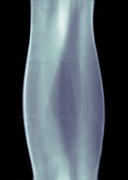
\includegraphics[width=5.560cm,height=8.000cm]{sinograms/unet2d.png}};
\end{scope}

\node[below=12pt,align=center,font=\small] at (out-nearsoutheast) {\textbf{Completed $\hat y$}\\$180\times128$};

\draw [connection]  (dec0-east)    -- node {\midarrow} (head-west);

\draw [connection]  (head-east)    -- node {\midarrow} (sum-west);

\draw [connection]  (sum-east)    -- node {\midarrow} (dc-west);

\draw [connection]  (dc-east)    -- node {\midarrow} (out-west);

\draw[bus] ($(in-east)+(0.9,0)$) -- ++(0,-7.6) coordinate (bus) -- (bus -| sum-south)
    node[pos=0.5,below,font=\small,opacity=1] {measured sinogram $y$: residual learning and data consistency}
    -- (sum-south);
\draw[bus] (bus -| sum-south) -- (bus -| dc-south) -- (dc-south);

\begin{scope}[shift={($(in-west)+(0,-9.2)$)}]
\filldraw[fill=\ConvColor,fill opacity=0.7,draw=black!60] (0.0,0.0) rectangle ++(0.45,0.4);
\filldraw[fill=\ActColor,fill opacity=0.7,draw=black!60] (0.45,0.0) rectangle ++(0.15,0.4);
\node[anchor=west,font=\small] at (0.7,0.2) {conv $3\times3$ + InstanceNorm + LeakyReLU};
\filldraw[fill=\PoolColor,fill opacity=0.7,draw=black!60] (7.2,0.0) rectangle ++(0.6,0.4);
\node[anchor=west,font=\small] at (7.9,0.2) {max pooling $2\times2$};
\filldraw[fill=\UpColor,fill opacity=0.7,draw=black!60] (14.4,0.0) rectangle ++(0.6,0.4);
\node[anchor=west,font=\small] at (15.1,0.2) {bilinear $\times2$ + conv $3\times3$};
\filldraw[fill=\CopyColor,fill opacity=0.7,draw=black!60] (21.6,0.0) rectangle ++(0.6,0.4);
\node[anchor=west,font=\small] at (22.3,0.2) {skip connection (concatenation)};
\filldraw[fill=\OutColor,fill opacity=0.7,draw=black!60] (0.0,-0.8) rectangle ++(0.6,0.4);
\node[anchor=west,font=\small] at (0.7,-0.6000000000000001) {conv $1\times1$};
\shade[ball color=\SumColor] (7.5,-0.6000000000000001) circle (0.22);
\node[anchor=west,font=\small] at (7.9,-0.6000000000000001) {residual: $y + f_\theta(y)$};
\shade[ball color=\DCColor] (14.700000000000001,-0.6000000000000001) circle (0.22);
\node[anchor=west,font=\small] at (15.1,-0.6000000000000001) {data consistency (measured views kept)};
\draw[bus] (21.6,-0.6000000000000001) -- ++(0.6,0);
\node[anchor=west,font=\small] at (22.3,-0.6000000000000001) {copy of the input};
\end{scope}

\end{tikzpicture}
\end{document}
